\section{Wyzwania}

W związku z nietypowym podejściem do problemu, zarówno projekt, jak i implementacja C-=-1 przedstawiła szereg ciekawych wyzwań.
W szczególności są one powiązane z możliwością wykonywania różnego kodu w zależności od kontekstu uruchomienia oraz publiczną naturą reprezentacji pośredniej.

\subsection{Instancje generyków jako element modelu semantycznego}
\label{challenges:generic_instance_placement}
Jednym z wyzwań powiązanych z udostępnieniem reprezentacji pośredniej programiście, jest wybór lokalizacji w modelu semantycznym, w której będą umieszczane instancje generyków.
Instancja szablonu może zależeć od typów lub funkcji pochodzących z pakietów, które nie były dostępne w czasie kompilacji generyka.

Rysunek \ref{generic_packages_dependencies} zawiera diagram przedstawiający taki przypadek.
Pakiety \emph{A} oraz \emph{B} są od siebie niezależne.
W \emph{A} zdefiniowany został generyk \lstinline{List}, natomiast w \emph{B} jest typ \lstinline{Type}.
Pakiet \emph{C} zależy od \emph{A} i \emph{B} i używa szablonu \lstinline{List}, specjalizując, go przy użyciu \lstinline{Type}.
W ten sposób powstaje nowy typ: \lstinline{List<Type>}.
Umieszczenie tego nowego bytu w modelu semantycznym, nie naruszając jego spójności oraz w sposób zrozumiały dla programisty nie jest proste.

Na podstawie diagramu na rysunku \ref{generic_packages_dependencies} można zaproponować cztery miejsca, w których można umieścić instancję generyka.
Sytuacja tam przedstawiona jest najogólniejszym przypadkiem tego problemu, mając na uwadze, że dowolna kombinacja tych pakietów może być sobie równa (na przykład \emph{C} może być tym pakietem co \emph{A}), oraz że typów, od których zależy \lstinline{List}, może być więcej i mogą być zdefiniowane w różnych pakietach.
Miejsca, w których można umieścić instancję szablonu to: \begin{enumerate}
	\item \label{generic_location:A} Pakiet A.
	\item \label{generic_location:B} Pakiet B.
	\item \label{generic_location:C} Pakiet C.
	\item \label{generic_location:new} Nowy pakiet.
\end{enumerate}

Pakiety \emph{A} i \emph{B} łatwo odrzucić.
Jeśli umieścić instancję generyka w pakiecie \emph{B} to w przypadku, w którym pakiet \emph{A} z rysunku \ref{generic_packages_dependencies} zależałby od pakietu \emph{B}, stworzenie \lstinline{List<Type>} doprowadziłoby do zależności cyklicznej między pakietami.
Ponadto, jeśli generyk \lstinline{List} zależałby od typów z kilku różnych pakietów, to w którym z nich zawrzeć jego instancję, byłoby niejednoznaczne.
Umieszczanie instancji generyka w pakiecie \emph{A} prowadzi do analogicznych problemów.

Miejsce \ref{generic_location:C} w najprostszym przypadku (takim jak na rysunku \ref{generic_packages_dependencies}) może wydać się najlepsze.
Pakiet \emph{A} ma w końcu dostęp do wszystkich zależności \lstinline{List<Type>}.
Taka decyzja tworzy jednak problemy ze spójnością modelu przy bardziej złożonej strukturze zależności.
Rysunek \ref{generic_packages_dependencies:option:a} zawiera diagram sytuacji, w której występuje ten problem.
Pakiety \emph{C} oraz \emph{D} zależą od generyka z \emph{A} parametryzowanego typem z \emph{B}.
Ponieważ \emph{C} i \emph{D} są od siebie niezależne, w obydwu powstały instancje tego szablonu, oznaczone numerami 1 i 2.
Pakiet \emph{E}, pośrednio zależny od \lstinline{List<Type>}, nie może teraz jednoznacznie wyznaczyć, z której instancji skorzystać.
Nawet jeśli wprowadzić jakiegoś rodzaju mechanizm na rozwiązywanie takich konfliktów, spójność modelu semantycznego została naruszona i zostało wprowadzone źródło błędów programisty.

Miejsce \ref{generic_location:new} zostało ostatecznie wybrane jako najlepsze rozwiązanie tego problemu.
Instancje generyków są umieszczane w specjalnym pakiecie, istniejącym tylko na czas kompilacji.
Tworzy to pewne niespójności w modelu semantycznym, ponieważ ta biblioteka nie jest poprawnie zdefiniowana.
Nie zależy od żadnego innego pakietu, a wszystkie inne pakiety zależą od niej.
Te wyjątki do normalnej konstrukcji modelu semantycznego zostały przyjęte, aby przyśpieszyć implementację.
Rozwiązanie niezawierające takiego problemu zostało przedstawione na rysunku \ref{generic_location:new}.
Dla każdego pakietu zawierającego generyki generowany jest nowy pakiet, przechowujący wyłącznie ich instancje.
Ta nowa biblioteka, zależy od biblioteki deklarującej szablon oraz wszystkich pakietów, od których zależy instancja.
W ten sposób skonstruowany model semantyczny jest spójny i jasny dla programisty.

%todo: consistency formal proof?

\begin{figure}
	\caption{Diagram przykładowej relacji pomiędzy pakietami zawierającymi typ generyczny}
	\label{generic_packages_dependencies}
	\begin{center}
		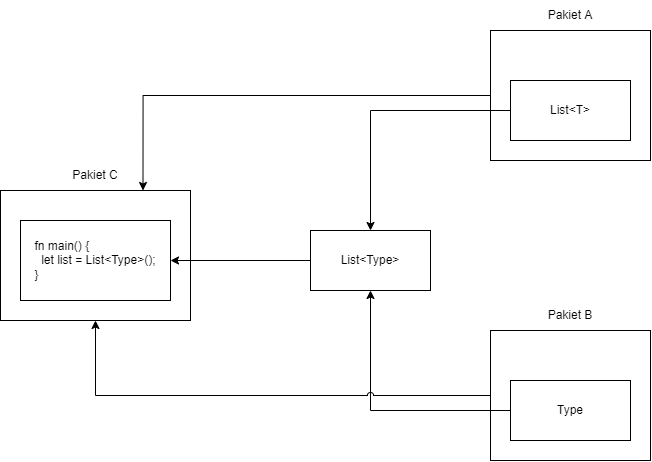
\includegraphics[width=\textwidth]{img/generic_misplaced.png}
	\end{center}
\end{figure}

\begin{figure}
	\caption{Diagram przykładowej relacji pomiędzy pakietami zawierającymi typ generyczny, przy umieszczaniu instancji w generującym pakiecie}
	\label{generic_packages_dependencies:option:a}
	\begin{center}
		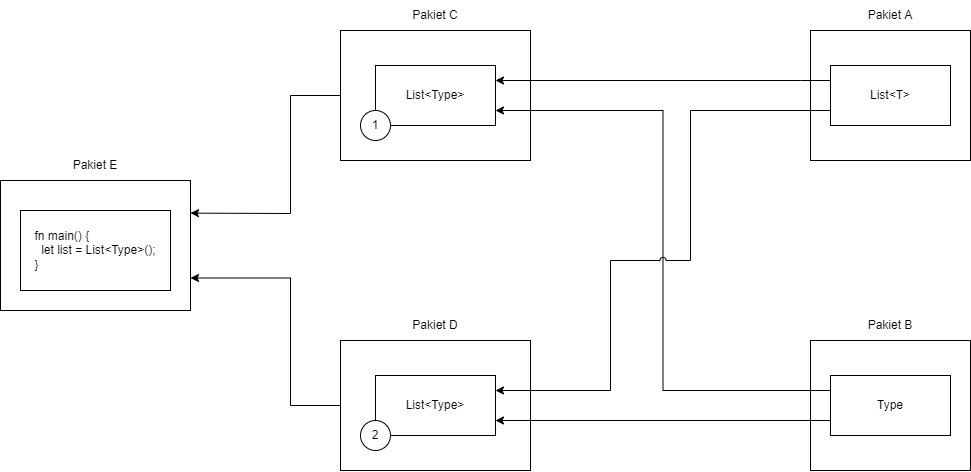
\includegraphics[width=\textwidth]{img/generics_placed_in_a.png}
	\end{center}
\end{figure}

\begin{figure}
	\caption{Diagram przykładowej relacji pomiędzy pakietami zawierającymi typ generyczny, przy umieszczaniu instancji w nowym pakiecie}
	\label{generic_packages_dependencies:option:new}
	\begin{center}
		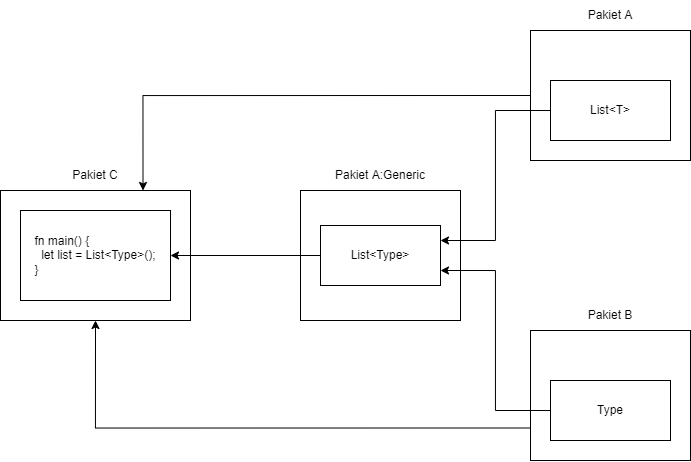
\includegraphics[width=\textwidth]{img/generics_placed_in_new.png}
	\end{center}
\end{figure}

\subsection{Kod wykonywany w fazie kompilacji}
O tym, czemu atrybuty są przetwarzane przed kodem i nie mogą używać funkcji z biblioteki, w której zostały zdefiniowane.

\subsection{Funkcje generyczne z ograniczeniami}
\label{challenges:generic_function_limitations}
Funkcje mogą być wykluczane z użycia w trakcie uruchomienia lub kompilacji. Jeśli generyk takiej funkcji zostanie stworzony z typem dalej ograniczającym wykonywalność tej funkcji, ona może być wykonywalna nigdy.

Na wczesnych etapach implementacji, instancje takich generyków były szczególnie problematyczne, ze względu na to jak rozwiązywanie przeciążeń jest zaimplementowane w C-=-1 (rozdział \ref{Function_overload_resolution}).
W związku z tym, w wypadku użycia funkcji generycznej, kompilator powołuje instancje wszystkich wersji tego szablonu, ze zgodną ilością parametrów.
Niektóre z nich, mogą być niepoprawne w danym kontekście. 

Na przykład operator \lstinline{new unique} został zdefiniowany w dwóch wersjach: na czas uruchomienia oraz kompilacji.
W czasie uruchomienia, odwołuje się on do funckji \lstinline{unsafe_new} która alokuje zadaną ilość bajtów na stercie.
W czasie kompilacji wywołuje funkcję generyczną \lstinline{compiletime_heap_allocate} która zwraca referencję na instancję zadanego typu.
Szczegóły zostały opisane w rozdziale \ref{operator_new}.

Sygnatury tych operatorów niczym się nie różnią.
Język rozpoznaje je jako oddzielne, rozróżnialne byty wyłącznie dlatego, że atrybuty którymi został adnotowane zmieniają ich dostępność w czasie kompilacji i uruchomienia.

Na wczesnych etapach implementacji, instancje funkcji generycznych były tworzone, przy założeniu, że ich kod będzie poprawny semantycznie.
Takie samo założenie obowiązuje przy tworzeniu zwykłych funkcji, ponieważ ze względu na ograniczenia czasowe, raportowanie o błędach kompilacji nie jest częścią pracy.
Kompilator najpierw kompletował reprezentację pośrednią instancji wszystkich wersji generyków pasujących do danego użycia.
Przy próbie dynamicznej alokacji typu, który nie mógł istnieć w czasie uruchomienia, takiego jak deskryptor funkcji, prowadziło to do odrzucenia poprawnego programu.

Naprawa tego problemu wymagała weryfikacji czy dana funkcja jest wykonywalna, w jakimkolwiek kontekście, po wykonaniu kodu powiązanych atrybutów.
Alternatywnym podejściem jest ignorowanie traktowanie błędów w instancji generyka, jako sygnał do odrzucenia tej specjalizacji, tak jak zostało to rozwiązane w C++ \cite{cppTemplatesCompleteGuide}.
Takie rozwiązanie mogłoby jednak prowadzić do zaśmiecania modelu semantycznego funkcjami, które nie mogą zostać użyte w żadnym kontekście i nie zawierały akurat żadnych błędów.
%todo: formalize?
\subsection{Operator new}
\label{operator_new}
Operator \lstinline{new} w C-=-1, tak jak w C++ służy do dynamicznej alokacji pamięci na stercie.

\subsection{Wybór przeciążenia funkcji}
\label{Function_overload_resolution}
To czy funkcja jest wykonywalna w czasie kompilacji albo uruchomienia można ustalić bardzo późno w trakcie budowy modelu semantycznego.

Na pytanie 'czy ta funkcja może być użyta w tym kontekście', kompilator jest w stanie odpowiedzieć dopiero kiedy wykonanły się na niej funkcje \lstinline{attach} wszystkich powiązanych z nią atrybutów.

%todo: example?

\subsection{Wyrażenia literałowe}

Wyrażenie literałowe przedstawia stałą wartość.
Na przykład w języku C++ \lstinline{int a = 4;} deklaruje i inicjalizuje zmienną a literałem 4.
Wyrażenia lietrałowe mogą reprezentować stałe różnych typów wbudowanych.
%todo: nameof, typeof

\subsection{Integracja z back-endem}
\label{backend_integration}
Przy pierwszym podejściu do budowy reprezentacji pośredniej, użyto dedykowanych struktur danych. Było to podejście najbardziej naturalne i dające najwięcej bezpieczeństwa dzięki silnemu typowaniu. Wszystkie struktury danych opisane w rozdziale \ref{reprezentacja_posrednia} miały powiązane ze sobą klasy C++.


To podejście tworzy jednak duży problem. Reprezentacja pośrednia musi zostać wyeksponowana użytkownikowi. Ponieważ nie istniała możliwość stworzenia binarnego interfejsu między kompilatorem a interpretowanym kodem, struktury danych CIR musiały być dodatkowo reprezentowane za pomocą struktur danych interpretera.


Użytkownik może dokonywać modyfikacji w CIR, co oznacza że może dojść do rozbieżności między strukturami danych interpretera a kompilatora. Utrzymywanie tych dwóch reprezentacji stanowiło poważne wyzwanie, dlatego postanowiono zmienić podejście. Użycie wyłącznie struktur danych interpretera do reprezentacji CIR usunęło ten problem, kosztem bezpieczeństwa kodu.


Ponieważ w nowym podejściu, z perspektywy C++ niemalże wszystkie obiekty miały ten sam typ, kompilator stracił możliwość statycznej weryfikacji kodu.
Aby zapewnić poprawność programu, koniecznym stało się dodawanie analizy argumentów do wszystkich funkcji.
